% LaTeX Präsentationsvorlage (2013) der TU Graz, rev12, 2013/01/31
\documentclass[aspectratio=169]{beamer}
% \documentclass[aspectratio=169]{beamer}
\usetheme{tugraz2013}
% \usetheme[notes]{tugraz2013}
% \usetheme[minimal]{tugraz2013}

%% Titelblatt-Einstellungen
\title[Mid-term presentation]{Mobile-Computing\\ Laboratory}
\author{Tobias Lafer}
% \date{Graz, XX. Dezember 2010}		% \today für heutiges Datum verwenden
\date{\today}
\institute[]{}
\instituteurl{https://www.tugraz.at/institute/iti/home/}
% \institutelogo{kurz.pdf}\right) 
% \additionallogo{institutslogo.pdf}

%%%%%%%%%%%%%%%%%%%%%%%%%%%%%%%%%%%%%%%%%%%%%%%%%%%%%%%%%%%%%%%%%%%%%%%%%%%%
\begin{document}
%%%%%%%%%%%%%%%%%%%%%%%%%%%%%%%%%%%%%%%%%%%%%%%%%%%%%%%%%%%%%%%%%%%%%%%%%%%%
\titleframe

\begin{frame}
  \frametitle{}
  \tableofcontents%[hideallsubsections] 
\end{frame}

\section{Overview}
\begin{frame}
	\frametitle{Overview}
	\begin{itemize}
		\item Option $1$
		\item \textbf{Activities}: Body-strenght exercises
		\begin{itemize}
			\item Periodic motions
			\item Quite unambiguous trajectory-profile
			\item $\Rightarrow$ Precise activity-classification possible even with simple algorithms (e.g. \textit{kNN})
		\end{itemize}
		\item Used Sensors:
		\begin{itemize}
			\item Accelerometer
			\item Gyroscope
		\end{itemize}
	\end{itemize}
\end{frame}

\begin{frame}
	\frametitle{Overview cont.}
	\begin{columns}[onlytextwidth]
		\begin{column}{0.75\textwidth}
			\begin{itemize}
				\item: \textbf{Used Phone}: LG Q6
				\begin{itemize}
					\item \textbf{Android-version:} $8.1.0$
					\item \textbf{Processor:} Qualcomm MS8940 (Octa-Core ARM Cortex A53)
					\item \textbf{RAM:} $2$ GB (only)
				\end{itemize} 
			\end{itemize}
		\end{column}
		\begin{column}{0.25\textwidth}
			\begin{center}
				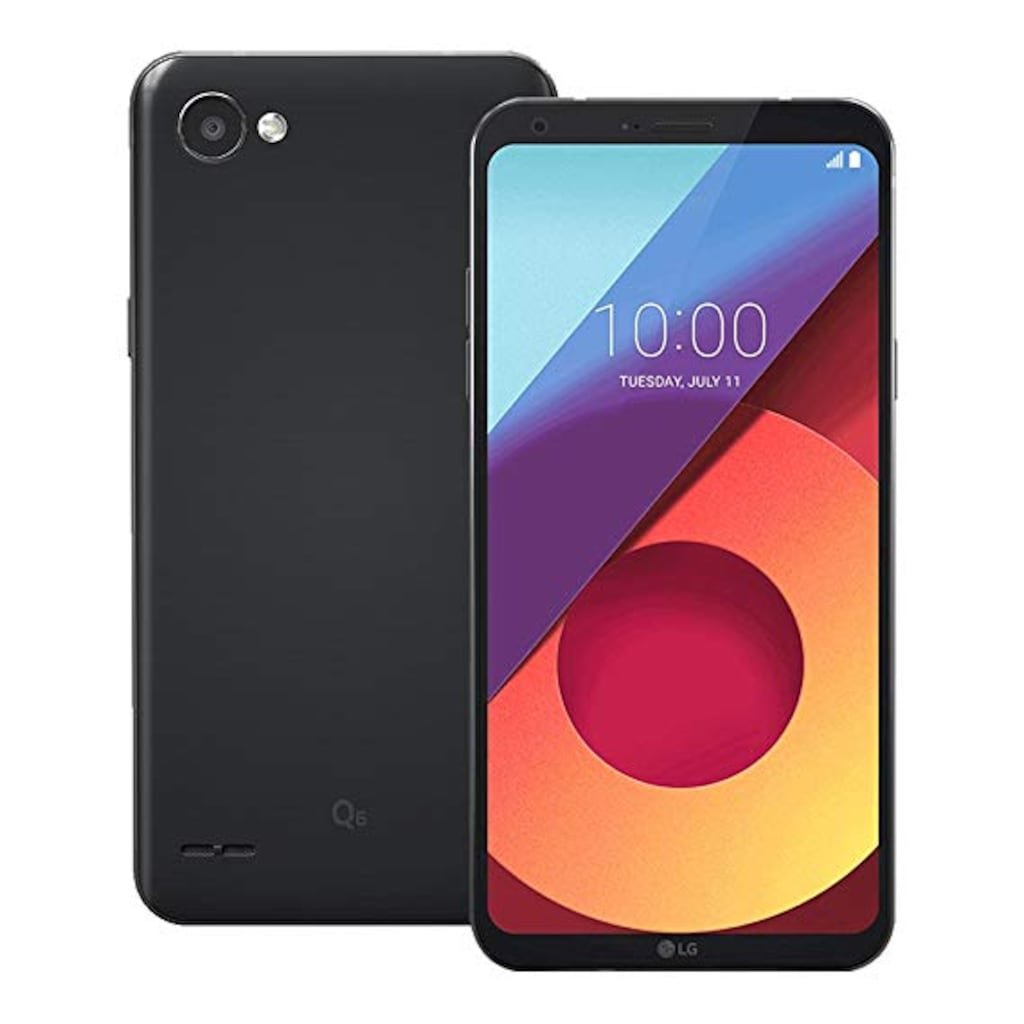
\includegraphics[width=\textwidth]{phone.jpeg}\\
				LG Q6
			\end{center}
		\end{column}
	\end{columns}
\end{frame}


\begin{frame}
	\frametitle{Current App-state}
	\vspace*{15pt}
	\begin{tabular}{p{0.5\textwidth}|p{0.5\textwidth}}
		\textbf{What is working} & \textbf{What is not working}\\
		\hline
		\begin{itemize}
			\item Data-Capturing
			\item Classification itself 
			\item Switching between (Android-)Activities
		\end{itemize} & 
		\begin{itemize}
			\item Interaction between Data-Capturing and Classification (Multi-threading issue)
			\item A "nice" UI
		\end{itemize}
	\end{tabular}
\end{frame}

\section{Data-Analysis and Signal-Processing}
\begin{frame}
	\frametitle{A closer look on the Activities}
	\begin{minipage}{0.49\textwidth}
		\centering
		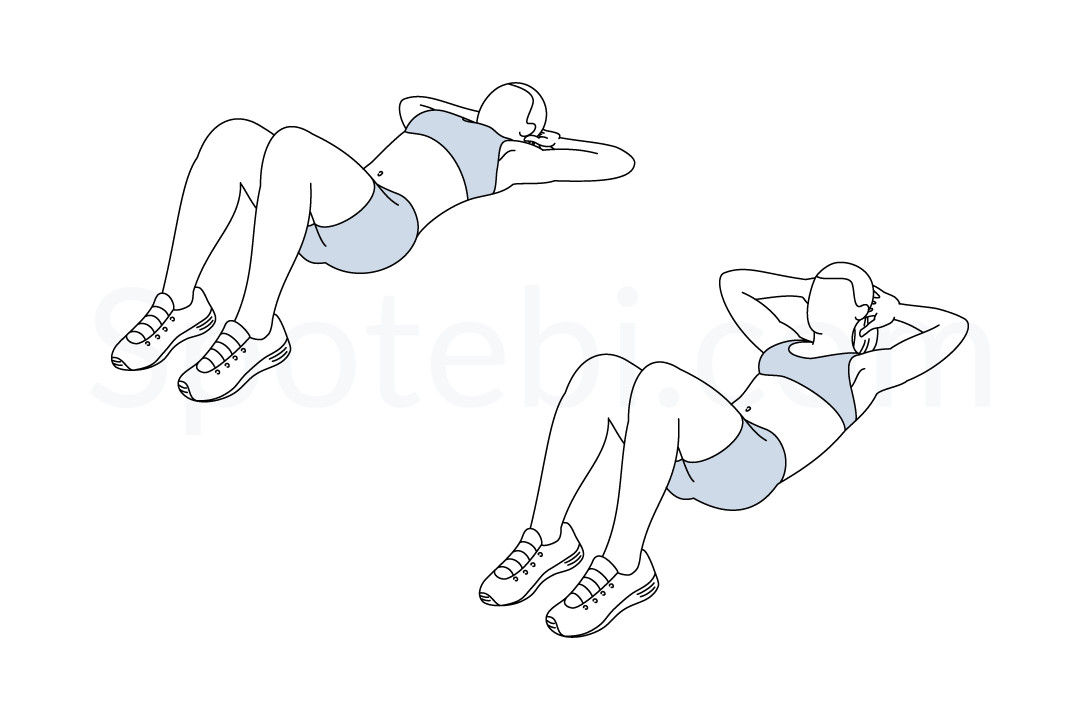
\includegraphics[width=0.4\textwidth]{crunches.jpeg}\\
		Crunches
	\end{minipage}\hfill
	\begin{minipage}{0.49\textwidth}
		\centering
		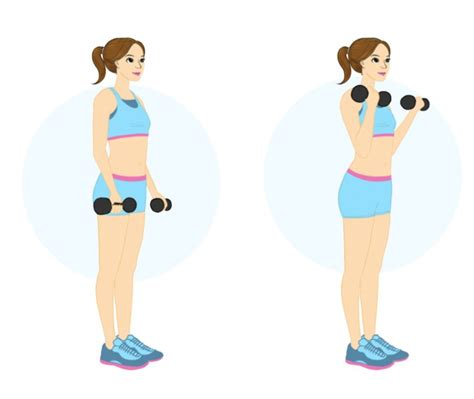
\includegraphics[width=0.4\textwidth]{curls.jpeg}\\
		Bizeps Curls
	\end{minipage}
	\begin{minipage}{0.49\textwidth}
		\centering
		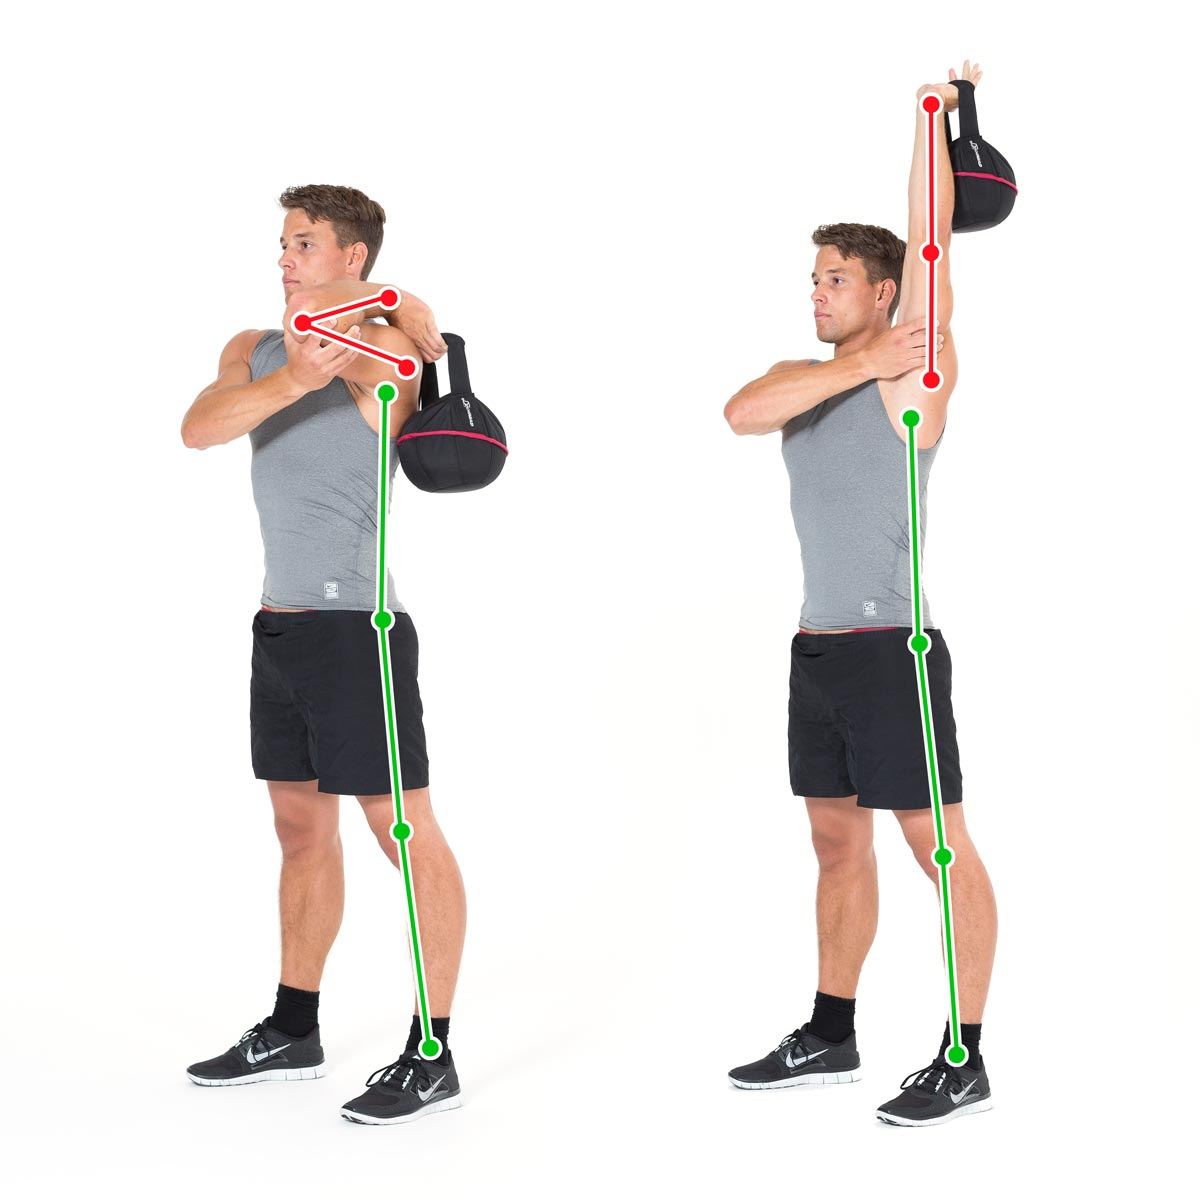
\includegraphics[width=0.4\textwidth]{triceps.jpeg}\\
		Triceps Curls
	\end{minipage} \hfill
	\begin{minipage}{0.49\textwidth}
		\centering
		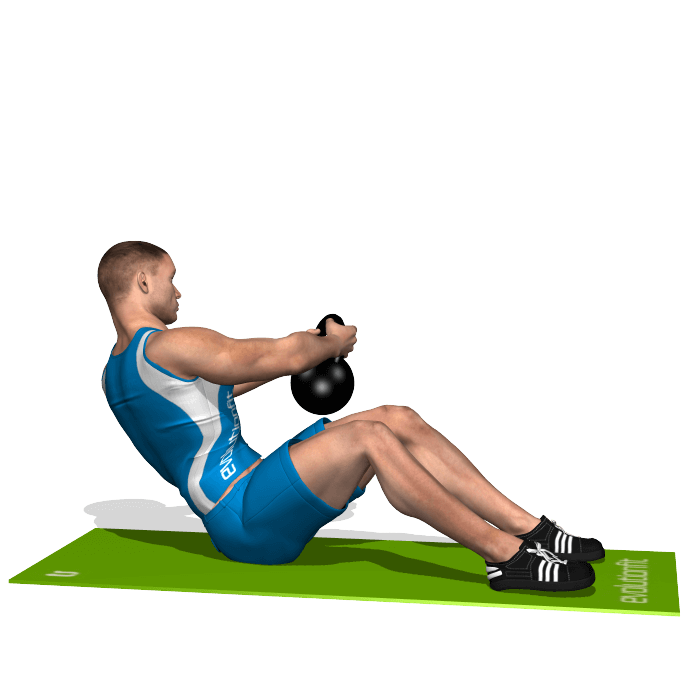
\includegraphics[width=0.4\textwidth]{russian_twist.png}\\
		Russian-Twist
	\end{minipage}
\end{frame}

\begin{frame}
	\frametitle{Activity-Characterization}
	\begin{columns}[onlytextwidth]
		\begin{column}{0.6\textwidth}
			\begin{itemize}
				\item Timeframes of $10$ seconds length
				\item Resampling to fixed sample-rate
				\item \textit{kNN}-classification by variance sensor-channels
				\begin{itemize}
					\item Currently $k=3$
					\item $\Rightarrow$ $6$ features ($x-, y-$ and $z-$ signal of each sensor)
				\end{itemize}
			\end{itemize}
		\end{column}
		\begin{column}{0.4\textwidth}
			\begin{center}
				\centering
				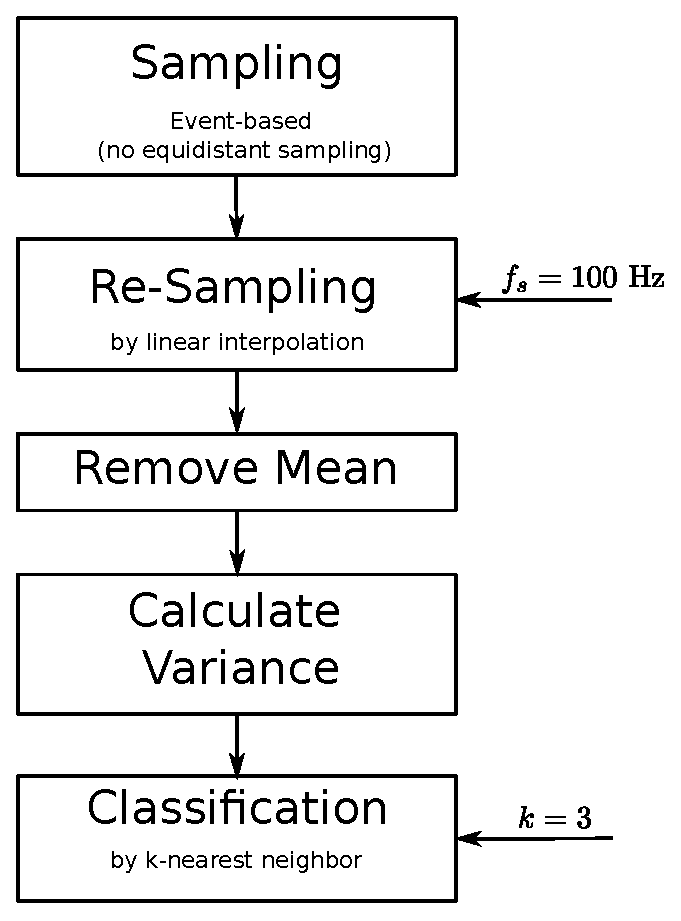
\includegraphics[width=0.7\textwidth]{signal_processing}
			\end{center}
		\end{column}
	\end{columns}
\end{frame}

\begin{frame}
	\frametitle{Features vs. Labels}
	\begin{itemize}
		\item $\approx 15$ samples for each activity in the 'training-set'
		\begin{itemize}
			\item Total timeframe used for variance calulation
			\item $\Rightarrow$ Noise-reduction
		\end{itemize}
		\item Test-Set:
		\begin{itemize}
			\item $3$ samples per activity
			\item Between $2$ and $3$ $10$ seconds-timeframes per sample
			\item $32$ test-set samples
		\end{itemize}
	\end{itemize}
\end{frame}

\section{Demo}
\sectionheader{Demo-Time}

\begin{frame}
	\frametitle{Thank you for your attention.}
\end{frame}

%%%%%%%%%%%%%%%%%%%%%%%%%%%%%%%%%%%%%%%%%%%%%%%%%%%%%%%%%%%%%%%%%%%%%%%%%%%%
\end{document}
%%%%%%%%%%%%%%%%%%%%%%%%%%%%%%%%%%%%%%%%%%%%%%%%%%%%%%%%%%%%%%%%%%%%%%%%%%%%

%% EOF
